% Lecture 1: Lagrangian (follow a tagged element) vs Eulerian (watch fixed points)
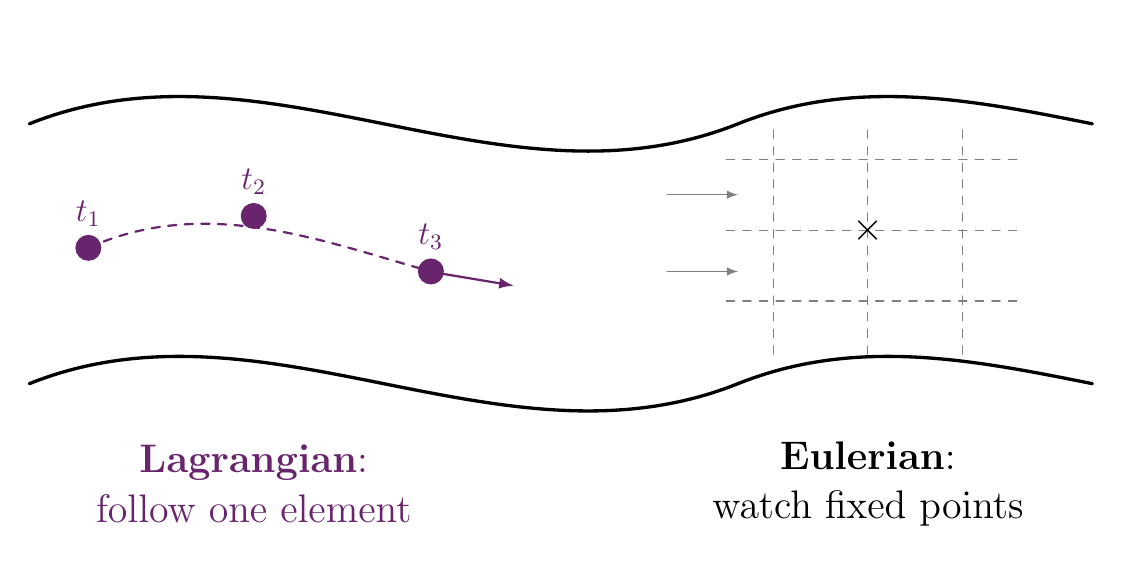
\begin{tikzpicture}[scale=1.5, >=latex, line cap=round]
  \definecolor{dpurple}{HTML}{68246D}
  \draw[very thick] (0,2.2) .. controls (2,3.0) and (4,1.4) .. (6,2.2) .. controls (7,2.6) and (8,2.4) .. (9,2.2);
  \draw[very thick] (0,0) .. controls (2,0.8) and (4,-0.8) .. (6,0) .. controls (7,0.4) and (8,0.2) .. (9,0);
  % Lagrangian: one element followed in time
  \draw[dpurple, dashed, thick] (0.5,1.15) .. controls (1.5,1.6) and (2.5,1.2) .. (3.4,0.95);
  \foreach \x/\y/\t in {0.5/1.15/t_1, 1.9/1.42/t_2, 3.4/0.95/t_3}{
    \fill[dpurple] (\x,\y) circle (0.11);
    \node[dpurple, font=\large, above] at (\x,\y+0.1) {$\t$};
  }
  \draw[->, thick, dpurple] (3.5,0.93) -- (4.1,0.83);
  \node[dpurple, font=\Large, align=center] at (1.9,-0.85) {\textbf{Lagrangian}:\\ follow one element};
  % Eulerian: fixed points in space
  \foreach \x in {6.3,7.1,7.9} \draw[gray, dashed] (\x,0.25) -- (\x,2.15);
  \foreach \y in {0.7,1.3,1.9} \draw[gray, dashed] (5.9,\y) -- (8.4,\y);
  \node[very thick] at (7.1,1.3) {\Large$\times$};
  \foreach \y in {0.95,1.6} \draw[->, gray] (5.4,\y) -- (6.0,\y);
  \node[font=\Large, align=center] at (7.1,-0.85) {\textbf{Eulerian}:\\ watch fixed points};
\end{tikzpicture}
